
\section{Higher-Order Momentum Balance}
\label{sc:higher-order-mom}

\begin{figure}
  \begin{center}
    \includegraphics[width=0.65\columnwidth]{\dir/figs/GIS.eps}
   \end{center}
  \caption{Observation-based balance velocities for Greenland (left) and depth-averaged speed from higher-order CISM (right) with basal sliding coefficients optimized to match the balance velocities (after Price et al., $PNAS$, \textbf{108}(22), 2011).}
  \label{fig:GIS_PNAS}
\end{figure} 

The higher-order dynamics scheme currently implemented in CISM (some output from which is shown in Figure \ref{fig:GIS_PNAS}) is discussed in more detail in the following sections. First, the derivation of the equations themselves is discussed, followed by a discussion and derivation of the boundary conditions. Generic solution methods for the nonlinear system of equations are then discussed. Finally, there is a brief discussion on the solution of the thickness evolution equation, which as noted above requires a different approach than in shallow-ice models.

\subsection{Derivation of the Blatter-Pattyn Equations}

The higher-order dynamics scheme implemented in CISM is based on the so-called Blatter-Pattyn model. The starting point for this model is the full Stokes equations

\begin{align*}
  & x:\quad \frac{\partial \tau _{xx}}{\partial x}-\frac{\partial P}{\partial x}+\frac{\partial \tau _{xy}}{\partial y}+\frac{\partial \tau _{xz}}{\partial z}=0 \\ 
 & y:\quad \frac{\partial \tau _{yy}}{\partial y}-\frac{\partial P}{\partial y}+\frac{\partial \tau _{xy}}{\partial x}+\frac{\partial \tau _{yz}}{\partial z}=0 \\ 
 & z:\quad \frac{\partial \tau _{zz}}{\partial z}-\frac{\partial P}{\partial z}+\frac{\partial \tau _{zy}}{\partial y}+\frac{\partial \tau _{xz}}{\partial x}=\rho g, \\ 
\end{align*}

where \textit{P} is the pressure and {\large \(\tau{}\)} is the deviatoric stress tensor. The latter is given by $\tau _{ij}=\sigma _{ij}+P\delta _{ij}$, 
where {\large \(\sigma{}\)} is the full stress tensor.

There are a number of ways to argue that, due to the shallowness of ice sheets (because the ratio of \textit{H}/\textit{L}, where \textit{H} is the thickness and \textit{L} is a relevant horizontal length scale, is small), the equations above can be reduced to the following first-order approximation:

\begin{align*}
  & x:\quad \frac{\partial \tau _{xx}}{\partial x}-\frac{\partial P}{\partial x}+\frac{\partial \tau _{xy}}{\partial y}+\frac{\partial \tau _{xz}}{\partial z}=0 \\ 
 & y:\quad \frac{\partial \tau _{yy}}{\partial y}-\frac{\partial P}{\partial y}+\frac{\partial \tau _{xy}}{\partial x}+\frac{\partial \tau _{yz}}{\partial z}=0 \\ 
 & z:\quad \frac{\partial \tau _{zz}}{\partial z}-\frac{\partial P}{\partial z}=\rho g \\ 
\end{align*}

The arguments that support this reduction are fairly complex, either based on a variational analysis or an asymptotic analysis. Two of the papers given in the references below ({\textit{Dukowicz et al.}, 2010}; {\textit{Schoof and Hindmarsh}, 2010}) provide more details on the mathematical background that allows us to state that these equations are first-order accurate approximations to the Stokes equations. 

We continue by noting that the 3rd (vertical) balance equation above can be integrated through the depth of the ice sheet to give an expression for the pressure, $P=\rho g\left( s-z \right)+\tau _{zz}(z)$

This is simply a statement the the full vertical normal stress is balanced by the hydrostatic pressure (the so-called \textit{hydrostatic assumption}). This expression can be substituted into the horizontal pressure gradient terms above to remove pressure from the equations. For example, for the \textit{x} component of velocity we have

\begin{align*}
  & x:\quad \frac{\partial \tau _{xx}}{\partial x}+\frac{\partial \tau _{xy}}{\partial y}+\frac{\partial \tau _{xz}}{\partial z}=\frac{\partial P}{\partial x} \\ 
 & x:\quad \frac{\partial \tau _{xx}}{\partial x}+\frac{\partial \tau _{xy}}{\partial y}+\frac{\partial \tau _{xz}}{\partial z}=\frac{\partial }{\partial x}\left[ \rho g\left( s-z \right)+\tau _{zz}(z) \right] \\ 
 & x:\quad \frac{\partial \tau _{xx}}{\partial x}-\frac{\partial \tau _{zz}}{\partial x}+\frac{\partial \tau _{xy}}{\partial y}+\frac{\partial \tau _{xz}}{\partial z}=\rho g\frac{\partial s}{\partial x} \\ 
\end{align*}

Now we can use the incompressibility and stress-strain colinearity constraints to rewrite the vertical normal deviatoric stress in terms of horizontal normal deviatoric stresses. This allows us to write the horizontal balance equations in terms of horizontal stress gradients only. Again, for the \textit{x} direction we have

\begin{align*}
  & \tau _{zz}=-\tau _{xx}-\tau _{yy} \\ 
 & -\frac{\partial \tau _{zz}}{\partial x}=-\frac{\partial }{\partial x}\left( -\tau _{xx}-\tau _{yy} \right)=\frac{\partial \tau _{xx}}{\partial x}+\frac{\partial \tau _{yy}}{\partial x} \\ 
 & \frac{\partial \tau _{xx}}{\partial x}-\frac{\partial \tau _{zz}}{\partial x}+\frac{\partial \tau _{xy}}{\partial y}+\frac{\partial \tau _{xz}}{\partial z}=\rho g\frac{\partial s}{\partial x}\quad ...\text{becomes}... \\ 
 & 2\frac{\partial \tau _{xx}}{\partial x}+\frac{\partial \tau _{yy}}{\partial x}+\frac{\partial \tau _{xy}}{\partial y}+\frac{\partial \tau _{xz}}{\partial z}=\rho g\frac{\partial s}{\partial x}\quad  \\ 
\end{align*}

Note that at this point we have removed the vertical balance equation entirely; it has been incorporated into the horizontal balance equations using incompressibility. The horizontal balance equations are now: 

\begin{align*}
  & x:\quad 2\frac{\partial \tau _{xx}}{\partial x}+\frac{\partial \tau _{yy}}{\partial x}+\frac{\partial \tau _{xy}}{\partial y}+\frac{\partial \tau _{xz}}{\partial z}=\rho g\frac{\partial s}{\partial x}\quad  \\ 
 & y:\quad 2\frac{\partial \tau _{yy}}{\partial y}+\frac{\partial \tau _{xx}}{\partial y}+\frac{\partial \tau _{xy}}{\partial x}+\frac{\partial \tau _{yz}}{\partial z}=\rho g\frac{\partial s}{\partial y} \\ 
\end{align*}

Next, we want to write these equations in terms of velocities, since that is what we are ultimately solving for. The link between stress gradients and velocities is through the constitutive law for ice (here we'll assume Glen's law) -- relating strain rates to stresses -- and the definition of the strain rate tensor -- relating strain rates to velocity gradients.

\begin{align*}
  & 1.\quad \tau _{ij}=B\dot{\varepsilon }_{e}^{\frac{1-n}{n}}\dot{\varepsilon }_{ij},\quad B=B(T) \\ 
 & 2.\quad \dot{\varepsilon }_{ij}=\frac{1}{2}\left( \frac{\partial u_{i}}{\partial x_{j}}+\frac{\partial u_{j}}{\partial x_{i}} \right) \\ 
 & 3.\quad 2\dot{\varepsilon }_{e}=\dot{\varepsilon }_{ij}\dot{\varepsilon }_{ij} \\ 
 & 4.\quad \eta \equiv \frac{1}{2}B\dot{\varepsilon }_{e}^{\frac{1-n}{n}} \\ 
 & 5.\quad \tau _{ij}=2\eta \dot{\varepsilon }_{ij} \\ 
\end{align*}

In order, the four expressions above give: 

\begin{enumerate}
\item  Glen's flow law (actually, the inverse flow-law here) where $B(T) = A(T)^{\frac{1-n}{n}}$ is a temperature dependent pre-factor
\item  The definition of the strain rate tensor in terms of velocity gradients
\item  The definition of the effective strain rate, $\dot{\varepsilon }_{e}$, a norm of the strain rate tensor
\item  A definition for the "effective viscosity" (after rearranging some terms in (1))
\item  Items (1)-(4) allow us to write the relationship between stress and strain in a standard Newtonian way, but with a non-Newtonian (nonlinear) viscosity
\end{enumerate}

Now taking these definitions into our stress balance equations above and expanding in terms of strain rates, velocity gradients, and effective viscosities, we have (for the \textit{x} direction only):

\begin{align*}
  & x:\quad 2\frac{\partial \tau _{xx}}{\partial x}+\frac{\partial \tau _{yy}}{\partial x}+\frac{\partial \tau _{xy}}{\partial y}+\frac{\partial \tau _{xz}}{\partial z}=\rho g\frac{\partial s}{\partial x} \\ 
 & x:\quad 2\frac{\partial }{\partial x}\left( 2\eta \dot{\varepsilon }_{xx} \right)+\frac{\partial }{\partial x}\left( 2\eta \dot{\varepsilon }_{yy} \right)+\frac{\partial }{\partial y}\left( 2\eta \dot{\varepsilon }_{xy} \right)+\frac{\partial }{\partial z}\left( 2\eta \dot{\varepsilon }_{xz} \right)=\rho g\frac{\partial s}{\partial x} \\ 
 & x:\quad 4\frac{\partial }{\partial x}\left( \eta \frac{\partial u}{\partial x} \right)+2\frac{\partial }{\partial x}\left( \eta \frac{\partial v}{\partial y} \right)+\frac{\partial }{\partial y}\left[ \eta \left( \frac{\partial u}{\partial y}+\frac{\partial v}{\partial x} \right) \right]+\frac{\partial }{\partial z}\left( \eta \frac{\partial u}{\partial z} \right)=\rho g\frac{\partial s}{\partial x} \\ 
\end{align*}


An analogous expression describes the \textit{y} direction momentum balance equation. For actually solving the system of equations, it is advantageous to combine all \textit{v} gradient terms for the \textit{x} balance equation and move them to the right-hand side (and vice versa for the \textit{y} balance equation). This gives the final form of the equations to be discretized and solved:


\begin{align*}
  & x:\quad 4\frac{\partial }{\partial x}\left( \eta \frac{\partial u}{\partial x} \right)+\frac{\partial }{\partial y}\left( \eta \frac{\partial u}{\partial y} \right)+\frac{\partial }{\partial z}\left( \eta \frac{\partial u}{\partial z} \right)=-2\frac{\partial }{\partial x}\left( \eta \frac{\partial v}{\partial y} \right)-\frac{\partial }{\partial y}\left( \eta \frac{\partial v}{\partial x} \right)+\rho g\frac{\partial s}{\partial x} \\ 
 & y:\quad 4\frac{\partial }{\partial y}\left( \eta \frac{\partial v}{\partial y} \right)+\frac{\partial }{\partial x}\left( \eta \frac{\partial v}{\partial x} \right)+\frac{\partial }{\partial z}\left( \eta \frac{\partial v}{\partial z} \right)=-2\frac{\partial }{\partial y}\left( \eta \frac{\partial u}{\partial x} \right)-\frac{\partial }{\partial x}\left( \eta \frac{\partial u}{\partial y} \right)+\rho g\frac{\partial s}{\partial y} \\ 
\end{align*}

%\section{References}
%\begin{itemize}
%\item  \href{http://www.ingentaconnect.com/content/igsoc/jog/2010/00000056/00000197/art00010}{Dukowicz, J. K., S.F. Price, and W. H. Lipscomb. 2010. Consistent approximations for ice-sheet dynamics from a principle of least action. \textit{J. Glaciol.}, \textbf{56}(197).}
%\end{itemize}
%
%\begin{itemize}
%\item  \href{http://homepages.vub.ac.be/~fpattyn/papers/Pattyn2003_JGRB.pdf}{Pattyn, F. A new three-dimensional higher-order thermomechanical ice sheet model: Basic sensitivity, ice stream development, and ice flow across subglacial lakes, \textit{J. Geophys. Res.}, \textbf{108}(B8), 2003}.
%\end{itemize}
%
%\begin{itemize}
%\item  \href{http://qjmam.oxfordjournals.org/content/63/1/73.abstract}{Schoof, C. and R. Hindmarsh. Thin-film flows with wall slip: an asymptotic analysis of higher order glacier flow models. \textit{QJMAM} \textbf{63}(1), doi:10.1093/qjmam/hbp025}.
%\end{itemize}
%\end{document}